\chapter[Evita Raced: Declarative Metacompiler]{Evita Raced: Declarative Metacompiler}
\label{ch:evita}

Declarative Networking has the potential to expand the lessons and impact of
database technologies into new domains, while reviving interest in classical
database topics like recursive query processing that have received minimal
attention in recent years.  Yet our own system was entirely implemented in an
imperative programming language: the initial version of the P2 runtime was
implemented in C++~\cite{p2:sosp}.  We asked ourselves whether Codd's vision
applies to our own efforts: can declarative programming improve the
implementation of declarative systems?

In this chapter, we put declarative systems ``in the mirror'' by investigating
a declarative implementation of one key component in any relational database
system, the query compiler.  Specifically, we reimplemented the query
compiler of P2 as a {\em metacompiler}: a compiler (optimizer) for the P2
language, \OVERLOG, that is itself written in \OVERLOG.  We named the resulting
implementation ``Evita Raced.''\footnote{``Evita Raced'' is almost
``Declarative'' in the mirror, but as with the \OVERLOG language itself, it
makes some compromises on complete declarativity.} Using Evita Raced, we
extended P2 with a number of important query optimization techniques it
formerly lacked, and found that our declarative infrastructure made this quite
elegant and compact.  

The elegance of our approach was derived in part from the fact that many query
optimization techniques -- like many search algorithms -- are at heart
recursive algorithms, and therefore would benefit from a declarative approach
in much the same way as networking protocols.  Even non-recursive optimization
logic -- such as parts of the magic-sets algorithm presented in
Chapter~\ref{ch:magic} -- are simple enough to express in a declarative fashion
that abstracts away mechanistic details such as state cleanup (e.g., garbage
collection) and invariant enforcement via key constraints and materialized view
maintenance.
%the scheduling of data-parallel steps (e.g., scanning all rules in a program
%in parallel versus sequentially).

The remainder of this chapter is organized as follows.  We describe the
architecture of Evita Raced in Section~\ref{ch:evita:sec:compile}, which
involves compiling an \OVERLOG program into a relational representation.
Compiling code into data is necessary in order to then express compilation
steps (i.e., rewrites, optimizations) as queries.  In
Section~\ref{ch:evita:sec:catalog} we describe the schema of the compiled code,
which is packaged with a schema in a Metacompiler Catalog relation.  The
architecture of Evita Raced is described in Section~\ref{ch:evita:sec:arch},
which consists of a dataflow of compilation steps and a scheduler to determine
compilation step order.  A given compilation step is called a {\em stage},
which can be written in either C++ or \OVERLOG.
Section~\ref{ch:evita:sec:bootstrap} describes our four basic C++ stages,
which bootstrap the compiler into a state that permits the subsequent dynamic
installation of our \OVERLOG stages.  In Section~\ref{ch:evita:sec:delta}, we
present our first declarative compilation stage (packaged with Evita Raced):
the delta rewrite~\cite{loo-sigmod06}.  This is followed by
Section~\ref{ch:evita:sec:local}, which describes our \OVERLOG rules for
performing the localization rewrite~\cite{p2:sosp} on a set of distributed
(join) rules.  Some final thoughts on the Evita Raced architecture are
presented in Section~\ref{ch:evita:sec:summary}.

\section{Declarative Compilation}
\label{ch:evita:sec:compile}

Evita Raced is a compiler (i.e., query optimizer) for the \OVERLOG declarative
language that supports a runtime-extensible set of program rewrites and
optimizations, which are themselves expressed in \OVERLOG.  This
metacompilation approach is achieved by implementing optimization logic via
dataflow programs (query plans) running over a set of tables.  Two main
challenges must be addressed to make this work.  First, all compiler state --
including the internal representation of both declarative \OVERLOG programs and
imperative dataflow programs -- must be captured in a relational representation
so that it can be referenced and manipulated from \OVERLOG.  Second, the
(extensible) set of tasks involved in optimization must itself be coordinated
via a single dataflow program that can be executed by the P2 runtime engine.
In this section we describe the implementation of the Evita Raced framework,
including the schema of the compiler state, the basic structure of the Evita
Raced dataflow graph, and the basic dataflow fragments needed to bootstrap the
optimizer.

\begin{figure*}
\ssp
\begin{center}
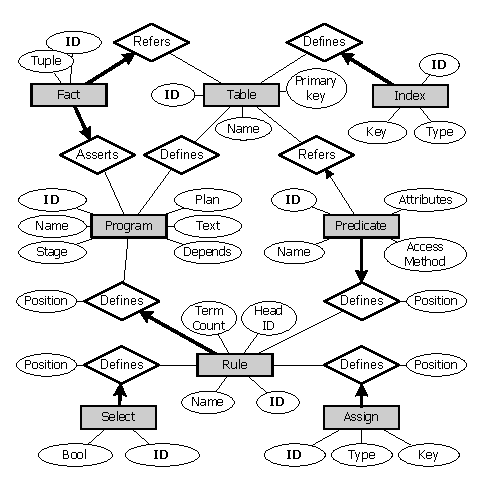
\includegraphics[scale=1.2]{figures/ERDiagram}
\caption{ER Diagram of a query plan in P2. The primary key columns shown in bold.}
\label{ch:evita:fig:p2er}
\end{center}
\end{figure*}

\subsection{Table-izing Optimizer State} 
\label{ch:evita:sec:catalog}

A typical query optimizer maintains a number of data structures to describe the
contents of a query, and to represent the ongoing state of a query planning
algorithm, including fragments of query plans.  Our first task in designing
Evita Raced was to capture this information in a relational schema.

Figure~\ref{ch:evita:fig:p2er} shows an Entity-Relationship diagram we
developed that captures the properties of an \OVERLOG program, and its
associated P2 dataflow query plans.  We derived the constraints in the diagram
by reviewing the semantic analysis rules enforced in the original P2 compiler;
we discuss a few of them here for illustration.  An \OVERLOG~{\em rule} must
appear in exactly one {\em program}.  A {\em select} term (e.g.,
\ol{f\_contains(X,P2) == false} in Figure~\ref{ch:p2:fig:overlogSP}) is a
Boolean expression over attributes in the predicates of the rule, and must
appear in exactly one {\em rule}.  The diagram indicates that a {\em predicate}
must also appear in a unique {\em rule}, and that it may possibly reference a
single {\em table}.  A predicate that references a table is called a {\em table
predicate} (or a \emph{materialized predicate}), while one that does not
reference a table is called an {\em event predicate}.  An {\em index} is
defined over exactly one {\em table}, and a {\em table} defines at least one
index (namely the primary key index, which P2 always constructs).  Some
relations may contain {\em facts} (input tuples) at startup, each of which must
belong to a single program and must reference a single table.

\begin{figure*}
\ssp
\begin{tabular}{|l|l|p{7cm}|} \hline
{\it Name}& {\it Description} & {\it Relevant attributes} \\ \hline\hline
table     & Table definitions & {\bf table\_id}, primary\_key\\ \hline
index     & Index definitions & {\bf index\_id}, {\bf table\_id}, keys, type \\ \hline
fact      & Fact definitions  & {\bf program\_id}, {\bf table\_id}, {\bf id}, tuple\\ \hline
program   & User program description     & {\bf program\_id}, name, stage, text, depends, plan \\ \hline
rule      & Rules appearing in a program   & {\bf program\_id}, {\bf rule\_id}, name,  term\_count, head\_id \\ \hline
predicate & Relational predicates  & {\bf id}, {\bf rule\_id}, table\_id, name, position, access\_method \\ \hline
select    & Selection predicates  & {\bf id}, {\bf rule\_id}, boolean, position \\  \hline
assign    & Variable substitution statements & {\bf id}, {\bf rule\_id}, variable, value, position \\ \hline 
\end{tabular}
\caption{The Metacompiler Catalog: tables defining an \OVERLOG program and dataflow execution plan.
         The primary key columns are shown in bold. }
\label{tbl:catalog}
\end{figure*}

The conversion from ER diagram to relational format was a textbook
exercise~\cite{DBTextbook}.  Table~\ref{tbl:catalog} lists the set of relations
that capture the entities mentioned in the ER diagram; we refer to this as the
{\em Metacompiler Catalog}.  We modified P2 to create these tables at system
startup, and they are accessible to any \OVERLOG programs (e.g., optimizations)
added to the system.
% In addition, there are compiler constraints that cannot be captured by key
% constraints alone.  For instance, a rule must contain exactly one head and
% one event predicate.  Such checks can be performed by integrity constraints
% written into the compiler logic (possibly as \OVERLOG programs).

\subsection{Metacompiler Architecture}
\label{ch:evita:sec:arch}
  
\begin{figure*}[htbp]
\centering
\ssp
\begin{tabular}{|p{2.5cm}|l|p{10cm}|} \hline
{\it Stage name}& {\it Language} & {\it Description} \\ \hline\hline
StageScheduler $(Section~\ref{ch:evita:sec:stageschedule})$ & C++ & 
Coordinates the compilation of stages.\\ \hline
Parser $(Section~\ref{ch:evita:sec:parser})$  & C++ & 
Bison based parser. Populates Metacompiler Catalog using program AST.\\ \hline
Planner $(Section~\ref{ch:evita:sec:planner})$ & C++ & 
Generates a dataflow description from the program data contained in the Metacompiler Catalog.\\ \hline
Installer $(Section~\ref{ch:evita:sec:installer})$ & C++  & 
Instantiates C++ dataflow objects from a dataflow description. \\ \hline
Delta Rewrite $(Section~\ref{ch:evita:sec:delta})$ & \OVERLOG & 
Converts rules based on materialized tables into an ECA form. \\ \hline
Localization $(Section~\ref{ch:evita:sec:local})$ & \OVERLOG   & 
Rewrites rules containing a distributed joins into a  localized form. \\ \hline
Magic-sets $(Chapter~\ref{ch:magic})$  & \OVERLOG & 
Rewrites rules to include magic predicates, which act as selection predicates for constants contained in query predicates. \\ \hline
System~R $(Section~\ref{ch:opt:sec:systemr})$ & \OVERLOG  & 
Performs System R dynamic programming optimization on all rules. \\ \hline
Cascades $(Section~\ref{ch:opt:sec:cascades})$ & \OVERLOG  & 
Query optimization based on a top-down search strategy. \\  \hline
%Debug print & \OVERLOG & 
%Add special pretty printer predicates, interposed in certain rules. The Planner stage 
%translates these printer predicates into dataflow objects that print the tuples
%that pass through. \\ \hline
\end{tabular} 
\caption{Primary Evita Raced compiler stages. }
\label{tbl:stages}
\end{figure*}
  

Optimization logic expressed in \OVERLOG is declarative, and Evita Raced
realizes this logic by converting it to a dataflow program to be executed by
the P2 dataflow subsystem, which was described in Section~\ref{ch:p2:sec:p2}.
In this section we describe how Evita Raced represents query optimization
programs as dataflow, and also the way it orchestrates multiple different
optimization programs through the P2 dataflow framework.

An optimizer built using Evita Raced is composed of an extensible number of
{\em stages}, each of which performs some compilation task on the input
program.  Table~\ref{tbl:stages} describes the primary compiler stages packaged
with the Evita Raced framework.  An Evita Raced stage can be written as a
dataflow program of one or more P2 elements in C++, which are then compiled
into the P2 binary; this is how we implement certain base stages required for
bootstrapping, further described in Section~\ref{ch:evita:sec:bootstrap}.  However,
the power of Evita Raced comes from its support for stages written in \OVERLOG,
which, in addition to being compactly expressed in a high-level language, can
be loaded into a running P2 installation at any time.

A stage programmer registers a new stage with Evita Raced by inserting a tuple
into the \ol{program} relation.  This tuple contains an unique identifier
($program\_id$), a name ($name$), a list of stage dependencies ($depends$), and
the program text ($text$).  Because the \ol{program} relation is used to convey
partial compilation results from stage to stage as well, \ol{program} tuples
also contain attributes for the name of the compiler stage currently operating
on the program ($stage$), and the final physical plan ($plan$), though these
attributes are empty when the programmer first creates the tuple.
Section~\ref{ch:evita:sec:stageschedule} describes the $depends$ attribute, and
its use in the installation of new stages.  The $plan$ attribute pertains to
the physical planner stage, which is described in
Section~\ref{ch:evita:sec:planner}.  We next describe the interfaces to an
Evita Raced compiler stage, after which we discuss the way that multiple such
stages are coordinated.

\subsubsection{The Stage API}
\label{ch:evita:sec:stages}

At base, an Evita Raced stage can be thought of as a stream query that listens
for a tuple to arrive on an event stream called \ol{<stage>::programEvent},
where \ol{<stage>} is the name of the stage.  The \ol{<stage>::programEvent}
table contains all the attributes mentioned in the \ol{program} table.  When
such a tuple arrives, the queries that make up that stage execute, typically by
modifying catalog tables in some way.  When a stage competes it inserts a new
\ol{program} tuple, containing the name of the stage in the $stage$ attribute,
into the program table.

To represent this behavior in a stage written in \OVERLOG, a relatively simple
template can be followed.  An \OVERLOG stage must have at least one rule body
containing the \ol{<stage>::programEvent} predicate.  This represents the
ability of the stage to react to new programs arriving at the system.  In
addition, the stage must have at least one rule that inserts a \ol{program}
tuple into the \ol{program} table to signal stage completion.

\subsubsection{Stage Scheduling}
\label{ch:evita:sec:stageschedule}

In many cases, optimization stages need to be ordered in a particular way for
compilation to succeed.  For example, a {\em Parser} stage must run before any
other stages, in order to populate the Metacompiler Catalogs.  The {\em
Planner} must follow any stages written in \OVERLOG, since it is responsible
for translating the relational representation of a query into a dataflow
representation.  And finally, the {\em Installer} stage must follow the {\em
Planner}, since it instantiates dataflow specifications as P2 C++ elements, and
installs them into the P2 runtime.  We will see other specific precedence
constraints in Section~\ref{ch:evita:sec:stages}.

A natural way to achieve such an ordering would be to ``wire up'' stages
explicitly so that predecessor stages directly produce
\ol{<stage>::programEvent} tuples for their successors, in an explicit chain of
stages.  However, it is awkward to modify such an explicit dataflow
configuration upon registration of new stages or precedence constraints.
Instead, Evita Raced captures precedence constraints as {\em data} within a
materialized relation called \ol{StageLattice}, which represents an arbitrary
partial order (i.e., an acyclic binary relation) among stages; this partial
order is intended to be a lattice, with the {\em Parser} as the source, and the
dataflow {\em Installer} as the sink.  
 
To achieve the dataflow connections among stages, the built-in {\em
StageScheduler} component (itself a stage) that listens for updates to the
\ol{program} table, indicating the arrival of a new \OVERLOG program or the
completion of a compiler stage for an on-going program compilation.  The {\em
StageScheduler} is responsible for shepherding compilation stage execution
according to the \ol{StageLattice}.  Given a \ol{program} update, the
StageScheduler ``joins with'' the \ol{StageLattic} to identify a next stage
that can be invoked, and derives a \ol{<stage>::programEvent} tuple that will
start the given stage; the contents (attributes) of the
\ol{<stage>::programEvent} tuple are the same as those in the updated
\ol{program} tuple.

\begin{figure*}[htbp]
\begin{center}
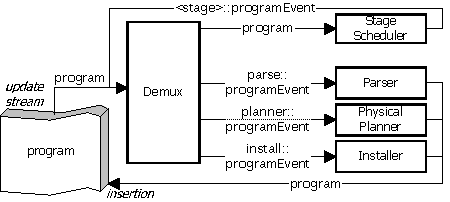
\includegraphics[scale=1.5]{figures/DefaultCompiler}
\ssp
\caption{The Evita Raced (cyclic) dataflow architecture, containing only the 
default compilation stages. We focus here on the portion of the P2 dataflow
that corresponds to the Evita Raced framework.}
\label{ch:evita:fig:basecompiler}
\end{center}
\end{figure*}

The StageScheduler and any compilation stages (whether built-in or
runtime-installed) are interconnected via the simple dataflow illustrated in
Figure~\ref{ch:evita:fig:basecompiler}.  The Evita Raced framework is embedded
in the same dataflow architecture used throughout the {\em Declarative
Networking} project.  As described in Section~\ref{ch:p2:sec:p2}
(and~\cite{p2:sosp}), the dataflow consists of a C++ ``demultiplexer'' that
routes tuples from its input (on the left) to individual event handlers
listening for particular tuple names (the arrows leaving the Demux element in
the figure contain the name of the tuple for which the stages to the right
listen).  The Evita Raced framework simply adds the its ``default stages'' to
the bootstrap routine of the P2 system.

Consider the simplicity of how the Evita Raced framework coexists with the P2
dataflow architecture.  To install a new (\OVERLOG) compilation stage into the
runtime, the Installer stage (Section~\ref{ch:evita:sec:installer}) simply extends
the {\em Demux} element to include a port for \ol{<stage>::programEvent}
tuples, routing them to the respective rule(s) of a given stage's \OVERLOG
program. The \ol{StageLattice} relation is also updated (e.g., through fact tuples
in the \OVERLOG stage program) to include its position in the compilation pipeline.
This completes the installation process, after which the \OVERLOG stage need only 
follow a simple protocol for when and how it should execute. 

The protocol to stage execution indicates when it should start (after receiving
a \ol{<stage>::programEvent} tuple) and what it must do on completion.  When a
stage completes, the only requirement is to update the \ol{program} table with
the ``stage'' attribute set to the stage name.  The {\em StageScheduler}
receives all such updates to the \ol{program} table -- see
Figure~\ref{ch:evita:fig:basecompiler}, the {\em Demux} \ol{program} tuple port
into the {\em StageScheduler} -- and uses the value of the \ol{program}
$depends$ attribute along with the \ol{StageLattice} relation to determine the
next stage.  This completes the full compilation process in Evita Raced of an
\OVERLOG program, from the {\em Parser} stage to the {\em Installer} stage, and
any other stages along the way.

To sum up, the life cycle of a program compilation starts when a user submits a
\ol{program} tuple to the system with a \ol{null} stage attribute.  The
StageScheduler receives that \ol{program} tuple and generates a
\ol{parse::programEvent} tuple (the Parser being the source stage in the
lattice), which is routed by the Demux element to the Parser stage.  When the
Parser is done, it updates that \ol{program} tuple in the corresponding table,
changing the tuple's $stage$ attribute to ``Parser.'' The StageScheduler
receives the \ol{program} tuple, and routes a \ol{planner::programEvent} to the
Demux and eventually the Physical Planner, which goes round the loop again to
the Installer.  Finally, once the Installer is done and notifies the
StageScheduler via a \ol{program} tuple with the $stage$ attribute set to
``Installer,'' the StageScheduler concludes the compilation process.  If the
\OVERLOG program being parsed is itself a new compilation stage, then after
installation, the scheduler updates the stage lattice.


\subsection{Compiler Bootstrapping}
\label{ch:evita:sec:bootstrap}

This section drills down on the stages that make up the baseline Evita Raced
compiler that is now part of P2's bootstrap routine.  As in many
metaprogramming settings, this is done by writing a small bootstrap component
in a lower-level language.  Evita Raced is initialized by a small C++ library
that constructs the cyclic dataflow of Figure~\ref{ch:evita:fig:basecompiler},
including the four default stages shown, which are themselves written in C++.
The bootstrap compiler is sufficient to compile simplified \OVERLOG programs
(local rules only, no optimizations) into operational P2 dataflows.  We next
describe the Parser, Planner, and Installer bootstrap stages in a bit more
detail, since they form the core foundation of the Evita Raced framework.

% \jmh{This paragraph was saved from a conflict with Tyson's checkin.  Joe will merge it in Tuesday night.
% The {\em stage scheduler} is a dataflow element that is responsible for providing the inputs to a 
% stage and processing any outputs from a stage. The input to a stage module is a tuple containing the 
% identifier of the program that it is responsible for
% processing. When the stage completes its task is will insert a new program tuple into
% the \ol{program} table with an updated $state$ attribute value that indicates (to the scheduler) the completion 
% of the stage operation on the input program. The program insertion triggers a new
% \ol{programEvent} tuple that is again directed to the stage scheduler, and the process repeats with
% the next scheduled stage in the compilation order. Stage execution order is determined by
% a relation of stage dependencies. The stage scheduler schedules
% a stage based on the dependency graph relation installed by the bootstrap process and the current 
% value of the $state$ attribute in the program tuple. The process completes when the program $state$ 
% attribute reaches stage that no other stage depends on.
% }


% \subsubsection{Default Query Compilation}
% 
% Figure~\ref{ch:evita:fig:basecompiler} shows a dataflow perspective of our default
% metacompiler. A user submits a new program to the system by inserting a tuple into the \ol{program} table.
% The program tuple contains initial values for all the attributes in the program table (see Table~\ref{tbl:tables}). 
% A program table insertion triggers a \ol{programEvent} event tuple that contains the program 
% identifier attribute value.  The "Demux" dataflow element routes the \ol{programEvent} tuple to the
% stage scheduler element, which determines the order in which a stages execute on the input
% program. 
% \petros{The job of the scheduler is a bit nebulous. Is there something
% you can say here to make clear what that does?}
% 
% 
% The input to a stage module is a tuple containing the identifier of the program that it is responsible for
% processing. When the stage completes its task is will insert a new program tuple into
% the \ol{program} table with an updated $State$ attribute value that indicates (to the scheduler) the completion 
% of the stage operation on the input program. The program insertion triggers a new
% \ol{programEvent} tuple that is directed to the stage scheduler, and the process repeats with
% the next scheduled stage in the compilation order. Stage execution order is determined by
% a relation of stage dependencies. The stage scheduler schedules
% a stage based on the dependency graph and the current value of the $State$ attribute in the program tuple. 
% The process completes when the program $State$ attribute reaches stage that no further stage depend on.
% 

\subsubsection{Parser}
\label{ch:evita:sec:parser}

The Parser passes the program text it receives in the \ol{programEvent}
through a traditional lexer/parser library specified using
flex~\cite{flexUrl} and bison\cite{bisonUrl}; this library code returns
a standard {\em abstract syntax tree} representation of the text.
Assuming the Parser does not raise an exception due to a syntax error,
it walks the abstract syntax tree, generating Metacompiler Catalog
tuples for each of the semantic elements of the tree. In addition to
recognizing the different terms of each rule, the parser also annotates
each term with its position in the given program.  By convention, the
first term of a rule body is the event predicate of the rule, if one
exists.  By the same convention, the zeroth term (position~$0$) for a
rule is the head predicate.



\subsubsection{Physical Planner}
\label{ch:evita:sec:planner}

The Physical Planner stage is responsible for doing a na\"{i}ve translation of
Metacompiler Catalog tuples (i.e., a parsed \OVERLOG program) into a dataflow
program.  It essentially takes each rule and deterministically translates it
into a dataflow graph language, based on the positions of terms in the rule.

More specifically, for each rule the Planner considers each term (predicate,
selection or assignment) in order of position attribute.  The predicate
representing the event stream is always planned first, and registers a listener
in the Demux element (recall Figure~\ref{ch:evita:fig:basecompiler}).  The
terms following the event stream are translated, left-to-right, into a C++
dataflow in the same way that the original P2 system did using
select-project-join operator methods.

We further mention three specific details.  First, whereas the original P2
system translated a logical query plan directly to a software dataflow
structure in C++, we have chosen to create an intermediate, textual
representation of the dataflow.  This representation is in a language akin to
the Click router's dataflow language, but we omit its details here.

Second, unlike the original P2 system, we have introduced a number of new join
methods for in-memory tables.  Prior to this work, P2 only supported
index-nested-loop joins, where the appropriate index was built on the join
column(s) during program compilation.  We have added to the P2 runtime, elements
for performing simple nested-loop join and sort-merge join methods.  Our
\ol{predicate} relation contains the choice of join method as one of its
attributes, and we have modified the P2 physical planner to create the
appropriate dataflow element that implements the given join method.

%% Those are naturally introduced to the P2 physical planner
%% machinery and otherwise
%% creates
%% a listening port in the P2 {\em Demux} on the event stream name. The predicates mentioned in the rule that
%% do not represent the event stream represent lookup operations (joins) on the referenced base relation.
%% A join operator is planned for a predicate by taking the input stream and schema and joining 
%% it - using the $access\_method$ given by the \ol{predicate} tuple - with a base relation producing a new tuple 
%% stream with the join schema. 
%% A selection term plans a filter operator that applies the $boolean$ attribute value to the input 
%% stream and passes only tuples that satisfy this expression to the output stream. \jmh{Again the "plans an operators that does X" doesn't mean much to me.}An assignment term 
%% plans a assignment operator that uses the input stream to evaluate the $value$ attribute (in the \ol{Assign}
%% tuple) to an atomic value. If the input stream contains an attribute named by $variable$ 
%% (in the \ol{Assign} tuple) then the value of that attribute is substituted in the input
%% stream, otherwise a new attribute is added to the input schema with the given value 
%% in the output stream. After all rule body terms have been planned, the planner adds a projection operator
%% that projects the output tuple stream onto the head predicate.

% generates a physical plan for each rule in a program. The execution order of a physical plan in 
% P2 is a leaf-to-root path, with the leaf corresponding to the event predicate and the root being the head 
% predicate. All predicates that lie in between the leaf and the root path are joined against the respective 
% base relation according to the access method given by the predicate tuple. 
% \petros{I would go as far as saying that the physical plan you derive is
% expressed in an operator language reminiscent of the Click
% language. Since we concentrate on logical plan manipulations here we
% don't go into details. The important thing to point out is that whatever
% you do is not tied to a particular runtime; one could take this physical
% plan and install it on a different runtime that isn't our dataflow but
% something else.}

% The initial operator is always the event predicate and it determines when the rule should fire. 
% If the rule does not contain an event predicate then a delta rewrite must be preformed on the rule. 
% The delta rewrite converts the original rule into a set of new rules
% that trigger whenever a side affect\petros{``side affect'' should be
%   ``side effect'' everywhere.} 
% occurs on a table predicate mentioned in the original rule. The delta rewrite is presented 
% in~\cite{boonSigmod}, and we fully adopt this rewrite in our metacompiler. The position attribute 
% defined by each predicate tuple determines the position of the corresponding physical operator in 
% the physical plan. Select and assign operators are also planned at the position indicated by the 
% respective table tuple.

Third, the Planner only understands rules that are in the
event-condition-action (ECA) form.  An \OVERLOG rule may have no event
predicate (e.g., ``\ol{table1 :- table2, table3.}'').  A {\em delta rewrite}
(from Loo, et al.~\cite{loo-sigmod06}) is used to convert such rules in an ECA
form (E.g., ``\ol{table1 :- delta\_table2, table3.}'' and ``\ol{table1 :-
table2, delta\_table3.}''.) As in~\cite{loo-sigmod06} \ol{delta\_table} denotes
a stream conveying insertions, deletions, or timeout refreshes to tuples of the
target \ol{table}.  We could have chosen to do this directly in the Planner,
but instead we built it as an \OVERLOG stage
(Section~\ref{ch:evita:sec:delta}).  This decision had an important
consequence; we could only use rules that contained an explicit event
predicate.  Furthermore, any \OVERLOG stage that contained rules with no
explicit event predicate depended on this compilation stage.  The delta rewrite
\OVERLOG stage consists of a mere $12$ rules ($25$ lines of code), and is
usually the first \OVERLOG stage to be compiled into the runtime.
 

\subsubsection{Plan Installer}
\label{ch:evita:sec:installer}

Given the output of the Physical Planner in the dataflow specification
language, what remains is to parse the textual representation of the dataflow,
construct the corresponding C++ elements, and ``wire them up'' accordingly.  We
have implemented this ``physical plan compiler'' in C++, and housed it within
the Installer stage.  Once these elements and their connections are
instantiated, the Plan Installer stage stitches them into the P2 runtime's
overall dataflow graph, as described in~\cite{p2:sosp}.  As noted
in~\ref{ch:evita:sec:compile}, this infrastructure made it easy for us to
extend P2 with the ability to modify its dataflow graph at runtime, a feature
not available prior to the release of Evita Raced.

% Since our focus here
% is on plan optimization, we omit the engineering
% details of that contribution.
% 


\subsection{Discussion}

The metacompilation approach of Evita Raced led us to naturally design the
system extensibility around issues of data storage and dataflow, rather than
library loading and control flow modifications.  While rule-based systems are
usually intended to be easier to extend than a procedural system, the internal
implementation of Evita Raced is especially elegant, due to our thorough
embrace of the native dataflow infrastructure, which we use both to execute
optimization code, and orchestrate stages via precedence tables and the
StageScheduler cycle.  The result of this design is that even a major addition
to the Evita Raced compiler entails very minimal modification to the runtime
state: only the addition of a pair of dataflow edges to connect up the new
stage, and the insertion of precedence tuples in a single table.  Beyond the
StageScheduler and the three bootstrap stages, no additional extensibility code
was added to P2 to support Evita Raced.

Despite its simplicity, Evita Raced is flexible enough that other researchers
have used it to enhance P2 with support for new languages at both its input and
output.  First, by extending the Parser element and registering some \OVERLOG
rules, Abadi and Loo were able to get P2 to optimize and rewrite programs
written in a new language, which extends \OVERLOG with the ability to attest to
the provenance of data in a manner similar to that of~\cite{abadi-netdb07}.
Second, Chu, et al. were able to use Evita Raced to cross-compile \OVERLOG programs
into dataflow specifications that execute on the DSN platform, a declarative
networking system that runs on wireless sensor nodes~\cite{chu-sensys07}.


\section{The Delta Rewrite}
\label{ch:evita:sec:delta}

In this section we describe our declarative implementation of the delta rewrite
for \OVERLOG rules.  The rewrite itself consists of a mere $12$ rules, which
includes rules for handling the Evita Raced API and cleanup rules that remove
rules that were rewritten, and therefore no longer needed. Before diving into
the specific rules for the rewrite we describe its actions by example.

\subsection{Delta by Example}

\begin{figure*}[!t]
\ssp
\centering
\begin{boxedminipage}{\linewidth}
{\bf materialize}(link,infinity,infinity,keys(1,2)). \\
{\bf materialize}(path,infinity,infinity,keys(1,2,3)).  \\
{\bf materialize}(shortestPath,infinity,infinity,keys(1,2,3)). \\
  
R1 {\bf path}(@X, Y, P, C) :- \\
\datalogspace {\bf link}(@X, Y, C), P := f\_cons(X, Y). \\
\\
R2 {\bf path}(@X, Y, P, C) :- \\
\datalogspace {\bf link}(@X, Z, C1), {\bf path}(@Z, Y, P2, C2),\\
\datalogspace f\_contains(X, P2) == false, \\
\datalogspace P := f\_cons(X, P2), C := C1 + C2. \\

R3 {\bf minCostPath}(@X, Y, a\_min$<$C$>$) :-  \\
\datalogspace {\bf path}(@X, Y, P, C). \\ 

R4 {\bf shortestPath}(@X, Y, P, C) :- \\
\datalogspace {\bf minCostPath}(@X, Y, C), {\bf path}(@X, Y, P, C).

\end{boxedminipage}
\caption{\label{ch:evita:fig:basicSP}Relevant rules copied from Figure~\ref{ch:p2:fig:overlogSP}.}
\end{figure*}

Consider the shortest path program in Figure~\ref{ch:evita:fig:basicSP} copied
over from Figure~\ref{ch:p2:fig:overlogSP}.  First thing to notice is the {\bf
materialize} statements at the top.  They indicate that non-zero lifetime
tables should exist for \ol{link}, \ol{path}, and \ol{shortestPath} tuples,
along with the appropriate primary key columns.  Since there is no {\bf
materialize} statement for the \ol{minCostPath} predicate, P2 considers such
tuple to be events, that will end up triggering rule~\ol{R4} when ``pulled''
from the event queue.  The question then is, what triggers the other rules to
produce \ol{minCostPath} event tuples.

\begin{figure*}[!t]
\ssp
\centering
\begin{boxedminipage}{\linewidth}
{\bf materialize}(link,infinity,infinity,keys(1,2)). \\
{\bf materialize}(path,infinity,infinity,keys(1,2,3)).  \\
{\bf materialize}(shortestPath,infinity,infinity,keys(1,2,3)). \\
  
R1 {\bf path}(@X, Y, P, C) :- \\
\datalogspace $\delta${\bf link}(@X, Y, C), P := f\_cons(X, Y). \\
\\
R2a {\bf path}(@X, Y, P, C) :- \\
\datalogspace $\delta${\bf link}(@X, Z, C1), {\bf path}(@Z, Y, P2, C2),\\
\datalogspace f\_contains(X, P2) == false, \\
\datalogspace P := f\_cons(X, P2), C := C1 + C2. \\

R2b {\bf path}(@X, Y, P, C) :- \\
\datalogspace $\delta${\bf path}(@Z, Y, P2, C2), {\bf link}(@X, Z, C1) \\
\datalogspace f\_contains(X, P2) == false, \\
\datalogspace P := f\_cons(X, P2), C := C1 + C2. \\


R3 {\bf minCostPath}(@X, Y, a\_min$<$C$>$) :-  \\
\datalogspace $\delta${\bf path}(@X, Y, P, C). \\ 

R4 {\bf shortestPath}(@X, Y, P, C) :- \\
\datalogspace {\bf minCostPath}(@X, Y, C), {\bf path}(@X, Y, P, C).

\end{boxedminipage}
\caption{\label{ch:evita:fig:basicSPDelta}Delta rewrite rules from Figure~\ref{ch:evita:fig:basicSP}.}
\end{figure*}

This is the purpose of the delta rewrite, which converts the rules in
Figure~\ref{ch:evita:fig:basicSP} into the rules shown in
Figure~\ref{ch:evita:fig:basicSPDelta}.  The $\delta$ predicate is shown (by
convention) at the front of the rule.  Since rule~\ol{R4} already contains an
{\emph event} predicate, it is planned to trigger off of \ol{minCostPath}
tuples, which is followed by a join with the \ol{path} relation, and then a
projection/insertion into the \ol{shortestPath} relation.  The remaining rules
are converted into $\delta$ form so that they can be installed into the P2
runtime by the $Planner$ stage.  We start with rule~\ol{R1}, which contains the
single subgoal \ol{link}.  The delta rewrite simply adds a delta annotation to
this predicate that informs the $Planner$ to trigger the rule when a
receive/insert/delete event occurs on the \ol{link} relation.  The same thing
happens with rule~\ol{R3} w.r.t., the \ol{plan} relation.

We come to rule~\ol{R2}, which has two subgoals \ol{link} and \ol{path}, both
of which are materialized tables.  In this case, we must break the rule into
two disjoint rules (one for each materialized subgoal).  The first of these
rules will trigger on (say) the \ol{link} tuple, followed by a join with
\ol{path} and selection (filter) on paths that overlap.  The second rule
triggers on \ol{path} event tuples, and join with the \ol{link} relation before
selecting out overlapping paths.  Both of these rules project any derivations
onto the \ol{path} relation, the write of which triggers further invocations
of rule~\ol{R2b}.

\subsection{Declarative Delta}

\begin{figure*}[!t]
\ssp
\centering
\begin{boxedminipage}{\linewidth}
/* Initiate a rewrite at position $1$ of a rule not already containing an event \\
   predicate in this position. */ \\
d1 {\bf rewrite}(@A, Pid, Rid, PredID, f\_idgen(), f\_idgen(), Pos) :- \\
\datalogspace {\bf delta::programEvent}(@A, Pid, \ldots), \\
\datalogspace {\bf sys::rule}(@A, Rid, Pid, \_, HeadID, \_, \_, \_, Goals), \\
\datalogspace {\bf sys::predicate}(@A, PredID, Rid, \_, Name, Tid, \_, Schema, Pos), \\
\datalogspace $Tid != null$, $Pos == 1$. \\

/* Initiate a rewrite position for each predicate in the rule body. */ \\
d2 {\bf rewrite}(@A, Pid, Rid, PredID, f\_idgen(), f\_idgen(), Pos) :- \\
\datalogspace {\bf rewrite}(@A, Pid, Rid, \ldots), \\
\datalogspace {\bf sys::predicate}(@A, PredID, Rid, \ldots, Schema, Pos), \\
\datalogspace $Pos > 1$. \\

\end{boxedminipage}
\caption{\label{ch:evita:fig:delta1}Deduce a rewrite fact for a new delta rule to be
created for a particular table predicate in the original rule's body.}
\end{figure*}

We now turn to the delta rewrite \OVERLOG stage used to produce the rules in
Figure~\ref{ch:evita:fig:basicSPDelta} from the rules in
Figure~\ref{ch:evita:fig:basicSP}.  Since no such stage exists prior to
installing this stage, all rules described here already contain an event
predicate, starting with the \ol{delta::programEvent} tuple.
Figure~\ref{ch:evita:fig:delta1} contains two rules that initiate the delta
rewrite by deducing a rewrite tuple for each rule in the target program.
Rule~\ol{d1} triggers off of a \ol{delta::programEvent} tuple, which contains
the target program identifier ($Pid$).  The rule ``joins with'' the \ol{rule}
and \ol{predicate} tables, selecting out the predicate in position~$1$ and
ensuring that predicate is not already an event, but rather a table predicate
($Tid\ !=\ null$).  Once a \ol{rewrite} event tuple has been deduced for a
given target rule, rule~\ol{d2} will initiate another rewrite event tuple for
each predicate in the target rule's body.  The $Pos > 1$ selection avoids the
head predicate (position $0$) and the first predicate already handled by
rule~\ol{d1}.

\begin{figure*}[!t]
\ssp
\centering
\begin{boxedminipage}{\linewidth}
/* Put the delta predicate in the first position of the new rule. */ \\
d3 {\bf sys::predicate}(@A, f\_idgen(), NewRid, Notin, Name, Tid, "DELTA", Schema, 1) :- \\
\datalogspace {\bf rewrite}(@A, Pid, Rid, DeltaPredID, NewRid, NewHeadID, \_), \\
\datalogspace {\bf sys::predicate}(@A, DeltaPredID, Rid, Notin, Name, Tid, ECA, Schema, Pos). \\

/* Make a new head predicate for the new rule by copying the old head predicate. */ \\
d4 {\bf sys::predicate}(@A, NewHeadID, NewRid, Notin, Name, Tid, ECA, Schema, 0) :- \\
\datalogspace {\bf rewrite}(@A, Pid, Rid, DeltaPredID, NewRid, NewHeadID, \_), \\
\datalogspace {\bf sys::rule}(@A, Rid, Pid, \_, HeadID, \ldots), \\
\datalogspace {\bf sys::predicate}(@A, HeadID, Rid, Notin, Name, Tid, ECA, Schema, \_).

\end{boxedminipage}
\caption{\label{ch:evita:fig:delta2}Rules that copy the old head predicate from the old rule
to the new rule, and creates the delta predicate in the new rule from the subgoal referenced
by the rewrite tuple.}
\end{figure*}

Assume we have initiated a rewrite tuple for a given rule $r$ and body
predicate $p_i$ at position~$i$.  The next step is to actually create the new
delta rule $\delta r$ with delta predicate $\delta p_i$ that references the
delta events of predicate $p_i$.  The new rule will take the following form
$h$~\ol{:-}~$\delta p_i, G_{j!=i}$, where $h$ references the original head predicate
in rule $r$ and $G_{j!=i}$ is the list of subgoals that exclude
predicate~$p_i$.

Figure~\ref{ch:evita:fig:delta2} contains two rules that create the head
predicate ($h$) and the delta predicate ($\delta p_i$) for the new delta rule
($\delta r$).  Rule~\ol{d3} creates the delta predicate, placing it in
position~$1$ (by convention) of the new rule and indicating that it is the
delta predicate for this rule.  Next, rule~\ol{d4} copies the head predicate
from the old rule by joining the old rule identifier ($Rid$) with the rule
table, and the predicate table along with the old head predicate identifier
($HeadID$).  The new head predicate will be given a new predicate identifier
($NewHeadID$) and a new rule identifier ($NewRid$).


\begin{figure*}[!t]
\ssp
\centering
\begin{boxedminipage}{\linewidth}
/* Kick off an iterator for the remaining rule subgoals. */ \\
d5 {\bf remainder}(@A, Pid, Rid, NewRid, 1, 2, Pos) :- \\
\datalogspace rewrite(@A, Pid, Rid, DeltaPredID, NewRid, \_, Pos). \\

/* Forward the remainder iterator along the subgoals. */ \\
d6 {\bf remainder}(@A, Pid, Rid, NewRid, $OldPos+1$, NewPos, DeltaPos) :- \\
\datalogspace {\bf remainder}(@A, Pid, Rid, NewRid, OldPos, NewPos, DeltaPos), \\
\datalogspace {\bf sys::rule}(@A, Rid, Pid, \ldots, Goals), \\
\datalogspace $OldPos < Goals$, \\
\datalogspace NewPos := $OldPos == DeltaPos$ ? NewPos : NewPos + 1. \\

/* Add the probe table to the rewritten rule. */ \\
d7 {\bf sys::predicate}(@A, f\_idgen(), NewRid, Notin, Name, Tid, "PROBE", Schema, NewPos) :- \\
\datalogspace remainder(@A, Pid, Rid, NewRid, Pos, NewPos, DeltaPos), \\
\datalogspace ::sys::predicate(@A, PredID, Rid, Notin, Name, Tid, \_, Schema, Pos), \\
\datalogspace $Pos != DeltaPos$. \\

/* Make a new assignement for the rewritten rule. */ \\
d8 {\bf sys::assign}(@A, f\_idgen(), NewRid, Var, Value, NewPos) :- \\
\datalogspace {\bf remainder}(@A, Pid, Rid, NewRid, OldPos, NewPos, \_), \\
\datalogspace {\bf sys::assign}(@A, Aid, Rid, Var, Value, OldPos). \\

/* Make a new selection for the rewritten rule. */ \\
d9 {\bf sys::select}(@A, f\_idgen(), NewRid, Bool, NewPos) :- \\
\datalogspace {\bf remainder}(@A, Pid, Rid, NewRid, OldPos, NewPos, \_), \\
\datalogspace {\bf sys::select}(@A, Sid, Rid, Bool, OldPos, AM).

\end{boxedminipage}
\caption{\label{ch:evita:fig:delta3}Rules that copy old subgoals to the new delta rule.}
\end{figure*}

Figure~\ref{ch:evita:fig:delta3} contains the next group of rules that copy the
body predicates from the old rule $r$ to the new $\delta r$ rule, excluding
predicate $p_i$.  We express this through a secondary group of event tuples,
called \ol{remainder}, that reference each of the desired body predicates.  A
\ol{remainder} tuple contains the predicate position relative to rule $r$ and a
new position in the $\delta r$ rule.  The new position must start at $2$, which
follows delta predicate.  Rule~\ol{d5} initiates the first \ol{remainder} tuple
from the \ol{rewrite} tuple and rule~\ol{d6} deduces a \ol{remainder} for each
subgoal the is to be copied to $\delta r$ rule.  Notice that rule~\ol{d6} does
not increment the $NewPos$ when $OldPos\ ==\ DeltaPos$.  The $DeltaPos$
position refers to the $p_i$ predicate in the original rule that will represent
the $\delta p$ predicate in the $\delta r$ rule.  If the $OldPos$ position
(relative to the original rule) is at the $DeltaPos$ position then we can reuse
this position for subsequent predicates $p_{j\ >\ i}$.

Recall that a subgoal can be either a predicate, a selection, or an assignment.
The remaining rules~\ol{d7, d8, d9} deal with copying each such goal from the
original rule~$r$ to the new $\delta r$ rule.  Rule~\ol{d7} skips the predicate
in $r$ that represents the $\delta p$ predicate in $\delta r$.  Again,
rule~\ol{d6} also considers this case when updating the new position.

\begin{figure*}[!t]
\ssp
\centering
\begin{boxedminipage}{\linewidth}
/* Create the new rule */ \\
d10 {\bf sys::rule}(@A, NewRid, Pid, Name, NewHeadID, null, Delete, Goals) :- \\
\datalogspace {\bf rewrite}(@A, Pid, Rid, DeltaPredID, NewRid, NewHeadID, Pos), \\
\datalogspace {\bf sys::predicate}(@A, DeltaPredID, Rid, \_, PredName, \ldots), \\
\datalogspace {\bf sys::rule}(@A, Rid, Pid, RuleName, \_, \_, Delete, Goals), \\
\datalogspace Name := RuleName + "delta" + PredName + Pos. \\

/* Clean up old rule state */ \\
d11 {\bf delete} {\bf sys::rule}(@A, Rid, Pid, Name, HeadID, P2DL, Delete, Goals) :- \\
\datalogspace {\bf rewrite}(@A, Pid, Rid, \ldots),  \\
\datalogspace {\bf sys::rule}(@A, Rid, Pid, Name, HeadID, P2DL, Delete, Goals). \\
  
/* Signal the completion of the delta rewrite to the $StageScheduler$. */ \\
d12 {\bf sys::program}(@A, Pid, Name, Rewrite, "delta", Text, Msg, P2DL, Src) :- \\
\datalogspace {\bf programEvent}(@A, Pid, Name, Rewrite, Status, Text, Msg, P2DL, Src).

\end{boxedminipage}
\caption{\label{ch:evita:fig:delta4}Creates a new rule tuple that references the delta 
rewrite rule. Cleans up the old (non-delta) rule. Inserts a program tuple indicating
that the delta rewrite has finished. }
\end{figure*}

The final set of rules are shown in Figure~\ref{ch:evita:fig:delta4}, which
represent the bookkeeping aspects of this rewrite.  Rule~\ol{d10} creates a
rule tuple that references the delta rule $\delta r$ for a given delta
predicate $\delta p_i$.  The old rule~$r$ is deleted by rule~\ol{d11}, which
through materialized maintenance will trigger the cleanup of the original head
predicate and subgoals.  Finally, rule~\ol{d12} inserts a \ol{program} tuple
that indicates the program has completed the delta rewrite stage.



\section{The Localization Rewrite}
\label{ch:evita:sec:local}

\begin{figure*}[!t]
\ssp
\centering
\begin{boxedminipage}{\linewidth}
R2a {\bf link\_copy}(@Z, X, Z, C1) :- \\
\datalogspace {\bf link}(@X, Z, C1). \\

R2b {\bf path}(@X, Y, P, C) :- \\
\datalogspace {\bf link\_copy}(@Z, X, Z, C1), {\bf path}(@Z, Y, P2, C2),\\
\datalogspace f\_contains(X, P2) == false, \\
\datalogspace P := f\_cons(X, P2), C := C1 + C2. \\

\end{boxedminipage}
\caption{\label{ch:evita:fig:basicSPLocal}The localized version of rule~\ol{R2} in
Figure~\ref{ch:evita:fig:basicSP}.}
\end{figure*}

Finally, we briefly describe the localization compiler stage, which turns a
rule with multiple location specifiers in its body to many rules, each of which
has a single location specifier in its body; this essentially turns a
distributed join into a set of local joins with partial result transmissions
among the rules involved~\cite{loo-sigmod06}.  This rewrite was part of the
original P2 system, but implemented in C++ and woven into the monolithic
compiler. 

We start with an example description using rule~\ol{R2} from
Figure~\ol{ch:evita:basicSP}.  This rule is rewritten into the two rules shown
in Figure~\ref{ch:evita:fig:basicSP}.  The \ol{link\_copy} predicate is an
{\emph event} predicate that copies the \ol{link} tuples at node $X$ to node
$Z$.  This will result in a network transfer if these attribute values are not
equal.  On node $Z$, the \ol{link\_copy} tuples will appear in rule~\ol{R2b}
and complete the condition of rule~\ol{R2}, sending the result back to node
$X$.

Declaratively, the localization stage traverses distributed rules in
left-to-right order starting with first body predicates (rules with local-only
body predicates are selected out early in the stage).  The location attribute
of the current predicate in this traversal is stored along with the cursor
information of the traversal.  A {\em breakpoint} is derived if the traversal
reaches a predicate with a location attribute that differs from the previous.
The breakpoint triggers a {\em split} rule at the given position, which creates
a new {\em glue} predicate $IR_copy$, and two new rules defined as follows.
\begin{CompactEnumerate} 
\item {\bf IR\_copy} :- (predicates to the left, excluding the breakpoint).  
\item (original rule head predicate) :- {\bf IR\_copy}, (predicates to the right, including
  the breakpoint).  
\end{CompactEnumerate} 
The location attribute in the {\bf IR\_copy} predicate is taken from the
predicate at the breakpoint position.  The other attributes in the {\bf
IR\_copy} predicate are taken from the predicates to the left of (and not
including) the breakpoint, which represents the schema of the intermediate
result prior to the breakpoint position predicate.  The algorithm then removes
the original rule, and moves recursively on the second rule, which is
considered the original rule in the above discussion.  The recursion terminates
at the rightmost predicate position.

The localization stage is not an optimization per se, but rather a program
rewrite necessary to make distributed rules executable.  The entire \OVERLOG
program for localization consists of only 12 rules.  The original P2 code that
performed this task in P2 consisted of approximately 400 lines of C++ scattered
throughout the entire ~$50414$ lines of code ($10794$ lines of .C files under
p2core alone).

\section{Summary} 
\label{ch:evita:sec:summary} 

The Evita Raced metacompilation framework allows \OVERLOG compilation tasks to
be written in \OVERLOG and executed in the P2 runtime engine.  It provides
significant extensibility via a relatively clean declarative language.  As we
will see next, many of the tasks of query optimization -- dynamic programming,
dependency-graph construction and analysis, statistics gathering -- appear to
be well served by a recursive query language.  The notion of metacompilation
also leads to a very tight implementation with significant reuse of code needed
for runtime processing.

One surprising lesson of our work was the breadth of utility afforded by the
metacompilation framework.  Although motivated by performance optimizations, we
have used Evita Raced for a number of unforeseen tasks.  These include:
automatically expanding user programs with instrumentation and monitoring
logic; generating pretty-printers for intermediate program forms; language
wrappers for secure networking functionality in the manner of
SecLog~\cite{abadi-netdb07}; stratification detectors and other static code
analysis.  None of these are performance optimizations per se, but all fit well
within an extensible, declarative program manipulation framework.  More
generally, we believe that metacompilation is a good design philosophy not only
for our work, but for the upcoming generation of declarative engines being
proposed in many fields.


